% Diagonal against a finite window of a supposed list of real decimals.
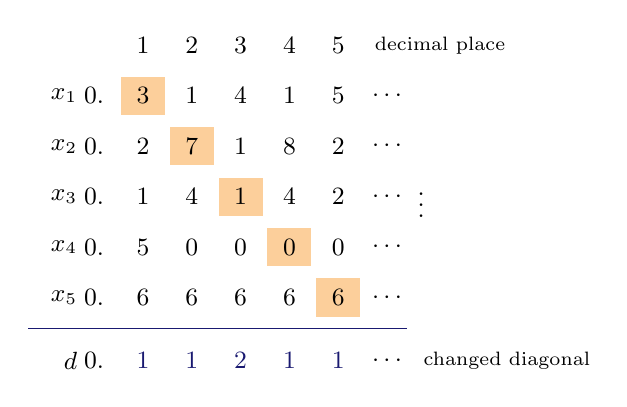
\begin{tikzpicture}[x=0.62cm,y=0.64cm,every node/.style={font=\small}]
  \node at (1,1) {$1$};
  \node at (2,1) {$2$};
  \node at (3,1) {$3$};
  \node at (4,1) {$4$};
  \node at (5,1) {$5$};
  \node[font=\scriptsize,anchor=west] at (5.55,1) {decimal place};
  % row x_1, diagonal digit 3
  \node[left] at (-0.15,0) {$x_1$};
  \node at (0,0) {$0.$};
  \fill[BurntOrange!35] (0.55,-0.38) rectangle (1.45,0.38);
  \node at (1,0) {$3$};
  \node at (2,0) {$1$};
  \node at (3,0) {$4$};
  \node at (4,0) {$1$};
  \node at (5,0) {$5$};
  \node at (6,0) {$\cdots$};
  % row x_2, diagonal digit 7
  \node[left] at (-0.15,-1) {$x_2$};
  \node at (0,-1) {$0.$};
  \node at (1,-1) {$2$};
  \fill[BurntOrange!35] (1.55,-1.38) rectangle (2.45,-0.62);
  \node at (2,-1) {$7$};
  \node at (3,-1) {$1$};
  \node at (4,-1) {$8$};
  \node at (5,-1) {$2$};
  \node at (6,-1) {$\cdots$};
  % row x_3, diagonal digit 1
  \node[left] at (-0.15,-2) {$x_3$};
  \node at (0,-2) {$0.$};
  \node at (1,-2) {$1$};
  \node at (2,-2) {$4$};
  \fill[BurntOrange!35] (2.55,-2.38) rectangle (3.45,-1.62);
  \node at (3,-2) {$1$};
  \node at (4,-2) {$4$};
  \node at (5,-2) {$2$};
  \node at (6,-2) {$\cdots$};
  % row x_4, diagonal digit 0
  \node[left] at (-0.15,-3) {$x_4$};
  \node at (0,-3) {$0.$};
  \node at (1,-3) {$5$};
  \node at (2,-3) {$0$};
  \node at (3,-3) {$0$};
  \fill[BurntOrange!35] (3.55,-3.38) rectangle (4.45,-2.62);
  \node at (4,-3) {$0$};
  \node at (5,-3) {$0$};
  \node at (6,-3) {$\cdots$};
  % row x_5, diagonal digit 6
  \node[left] at (-0.15,-4) {$x_5$};
  \node at (0,-4) {$0.$};
  \node at (1,-4) {$6$};
  \node at (2,-4) {$6$};
  \node at (3,-4) {$6$};
  \node at (4,-4) {$6$};
  \fill[BurntOrange!35] (4.55,-4.38) rectangle (5.45,-3.62);
  \node at (5,-4) {$6$};
  \node at (6,-4) {$\cdots$};
  \node at (6.7,-2) {$\vdots$};
  % the escaped real: 1 if the coral digit is not 1, and 2 if it is
  \draw[MidnightBlue,thin] (-1.35,-4.62)--(6.4,-4.62);
  \node[left] at (-0.15,-5.25) {$d$};
  \node at (0,-5.25) {$0.$};
  \node[MidnightBlue] at (1,-5.25) {$1$};
  \node[MidnightBlue] at (2,-5.25) {$1$};
  \node[MidnightBlue] at (3,-5.25) {$2$};
  \node[MidnightBlue] at (4,-5.25) {$1$};
  \node[MidnightBlue] at (5,-5.25) {$1$};
  \node at (6,-5.25) {$\cdots$};
  \node[font=\scriptsize,anchor=west] at (6.55,-5.25) {changed diagonal};
\end{tikzpicture}
